\begin{tikzpicture}
\node[inner sep=0,anchor=south west] (im) at (0,0) {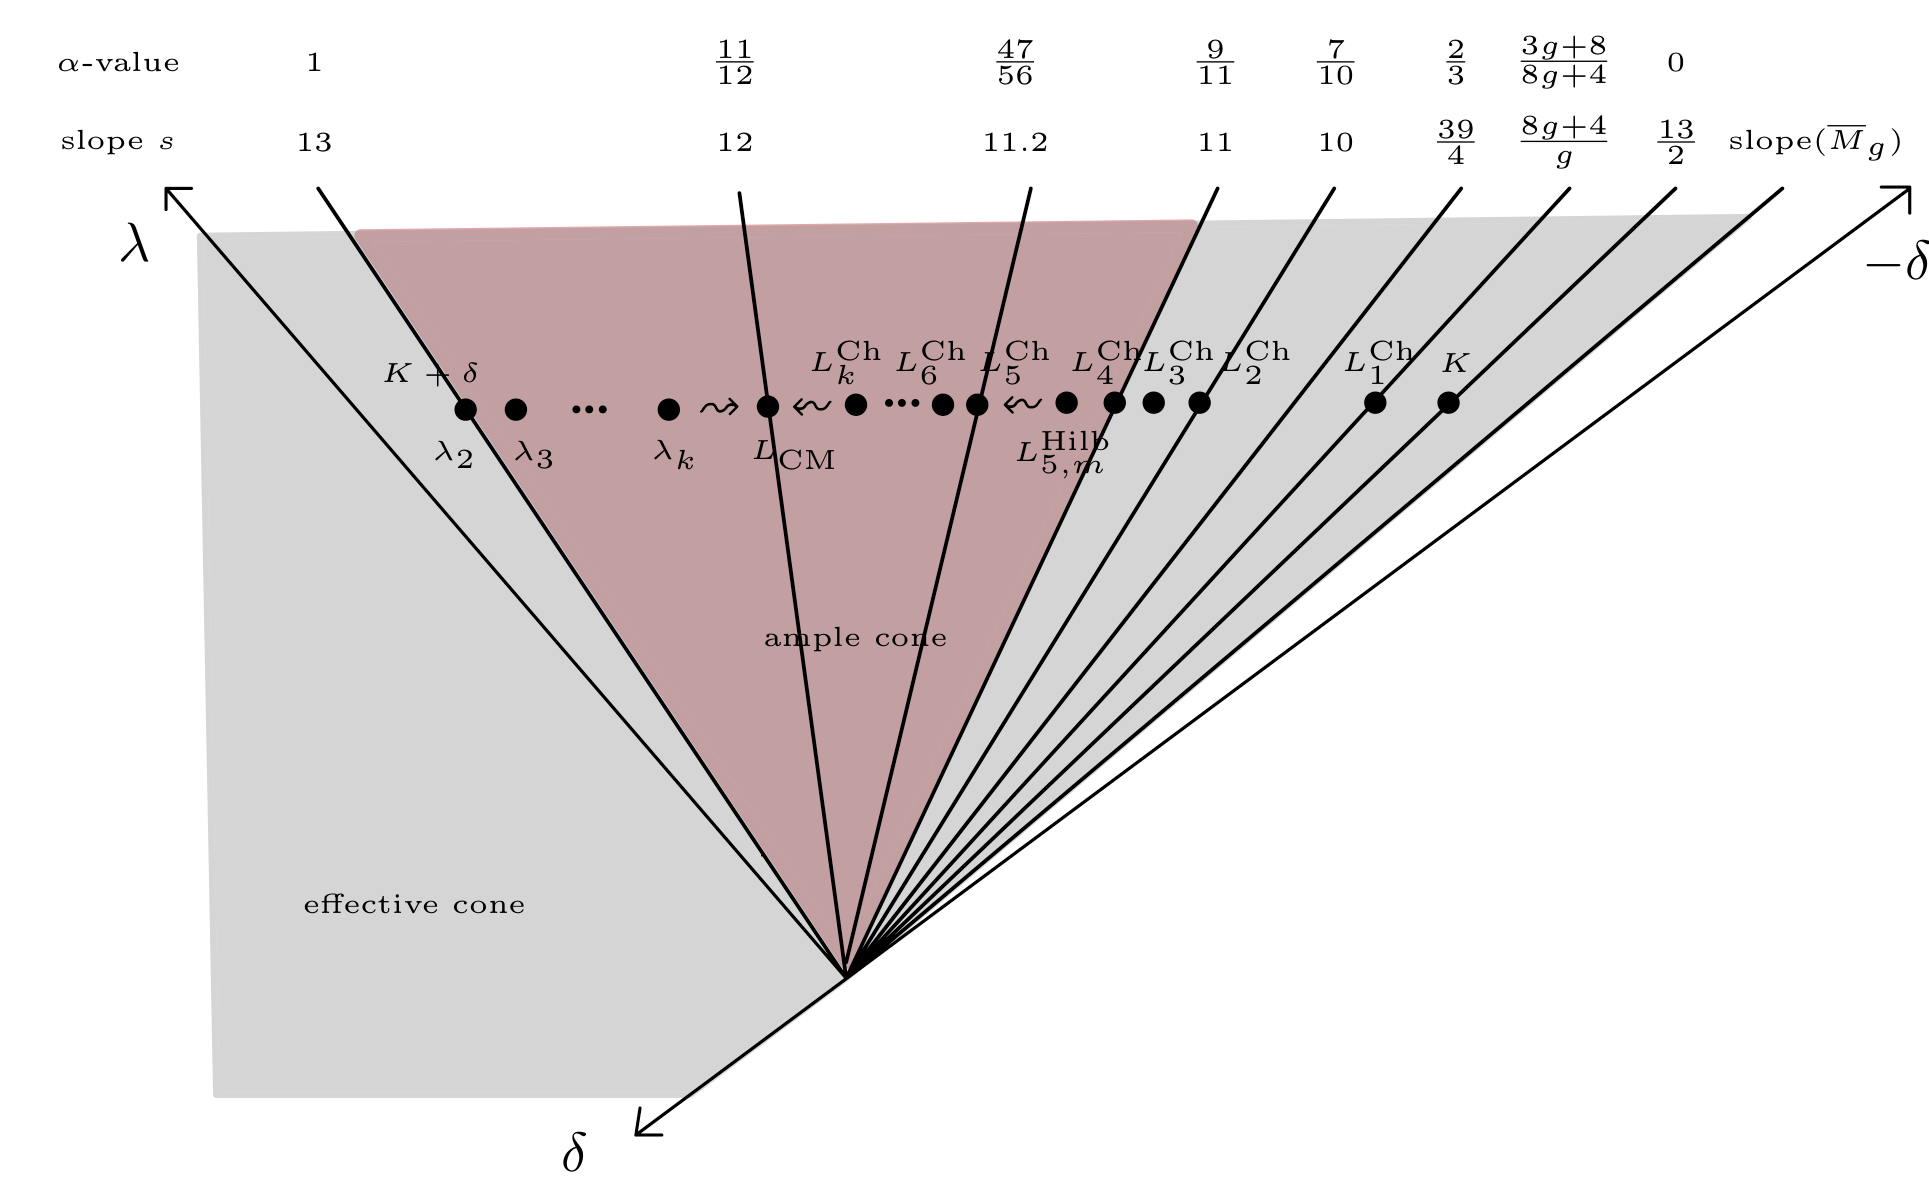
\includegraphics[width=.95\textwidth]{figures/moduli-cones.png}};
\begin{scope}[x={(im.south east)},y={(im.north west)}]
\fill[fill=white] (0.025937,0.964789) rectangle (0.096542,0.929577);
\node[font=\tiny,inner sep=0pt] at (0.061239,0.947183) {$\alpha$ 值};
\fill[fill=white] (0.027378,0.899061) rectangle (0.095101,0.862441);
\node[font=\tiny,inner sep=0pt] at (0.061239,0.880751) {斜率 $s$};
\fill[fill=white] (0.893372,0.899061) rectangle (0.991354,0.859155);
\node[font=\tiny,inner sep=0pt] at (0.942363,0.879108) {斜率 $(\overline M_g)$};
\fill[fill={rgb,255:red,213;green,213;blue,213}] (0.154179,0.252113) rectangle (0.275216,0.219249);
\node[font=\tiny,inner sep=0pt] at (0.214697,0.235681) {有效锥};
\fill[fill={rgb,255:red,194;green,159;blue,161}] (0.392507,0.477934) rectangle (0.494236,0.444601);
\node[font=\tiny,inner sep=0pt] at (0.443372,0.461268) {丰沛锥};
\end{scope}\end{tikzpicture}
